\documentclass[9pt]{beamer}
\usetheme{Boadilla}
\usepackage[utf8]{inputenc}
\usepackage{amsmath}
\usepackage{amsfonts}
\usepackage{amssymb}
\usepackage{graphicx}
\author{Adriano Del Vincio}
\title[Alpha 2]{Toy Model For Hyperfine Measurement}

\setbeamercolor{block title}{fg=white, bg = cyan }
\author[Adriano, Germano, Simone]{Adriano Del Vincio, Germano Bonomi,\\ Simone Stracka}
%\setbeamercovered{transparent} 
%\setbeamertemplate{navigation symbols}{} 
\logo{
\includegraphics[width = 0.125\textwidth]{../../logo/ALPHA_Logo.jpg}}
\newcommand{\nologo}{\setbeamertemplate{logo}{}}
\institute[]{University of Brescia, INFN Pisa} 
\titlegraphic{
\begin{figure}
\hspace{1.cm}

\includegraphics[width = 0.12\textwidth ]{../../logo/logounibs.png}
%\hspace{1cm}

\includegraphics[width = 0.25\textwidth ]{../../logo/1_Pisa_LOGO_SIGLA.pdf}
\end{figure}
} 
\begin{document}

\begin{frame}
\titlepage
\end{frame}

%\begin{frame}
%\tableofcontents
%\end{frame}


\begin{frame}{A brief introduction about the Monte Carlo}

This Monte Carlo produces two \texttt{.root} files, that are a simulated dataset of the hyperfine spectrum of anti-hydrogen.
\begin{figure}[hbtp]
 \centering
 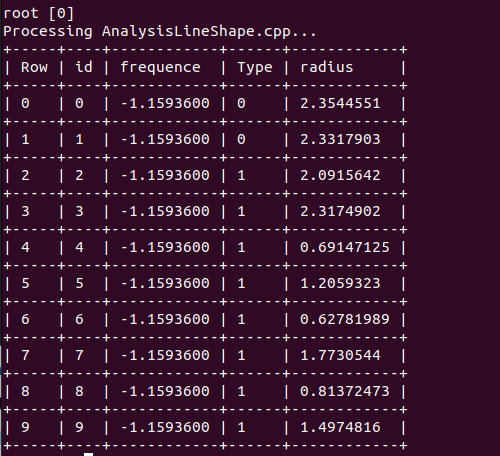
\includegraphics[width = 0.5\textwidth]{StructureDataTree.png}
 \caption{ Structure of the dataset.}
 \end{figure}

\end{frame}

\begin{frame}{A brief introduction about the Monte Carlo}

The Annihilation on the walls ($N_{mix}$) are generated using the two pdf of the transitions (c $\rightarrow$ b) and (d $\rightarrow$ a). The Annihilation on the residual gas ($N_{gas}$) are generated uniformly on the frequency spectrum. The definition of the important parameters of the simulation is in the following figure:

\begin{figure}[hbtp]
\centering
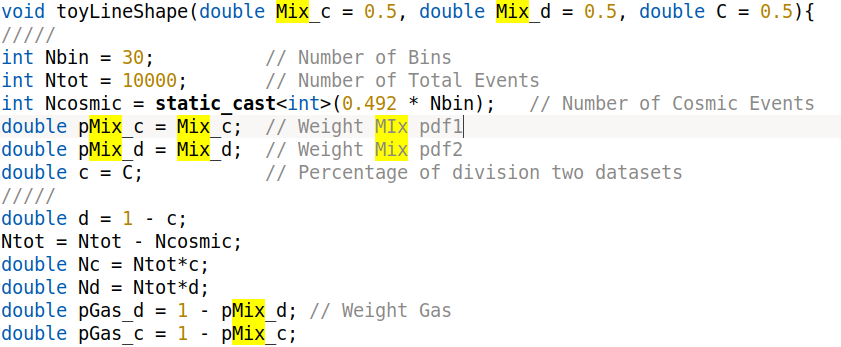
\includegraphics[width = \textwidth]{MontecarloParams.png}
\caption{ Parameter of the Montecarlo.}
\end{figure}


\end{frame}


\begin{frame}{Spline interpolation of the Spectrum.}
\begin{figure}[hbtp]
\centering
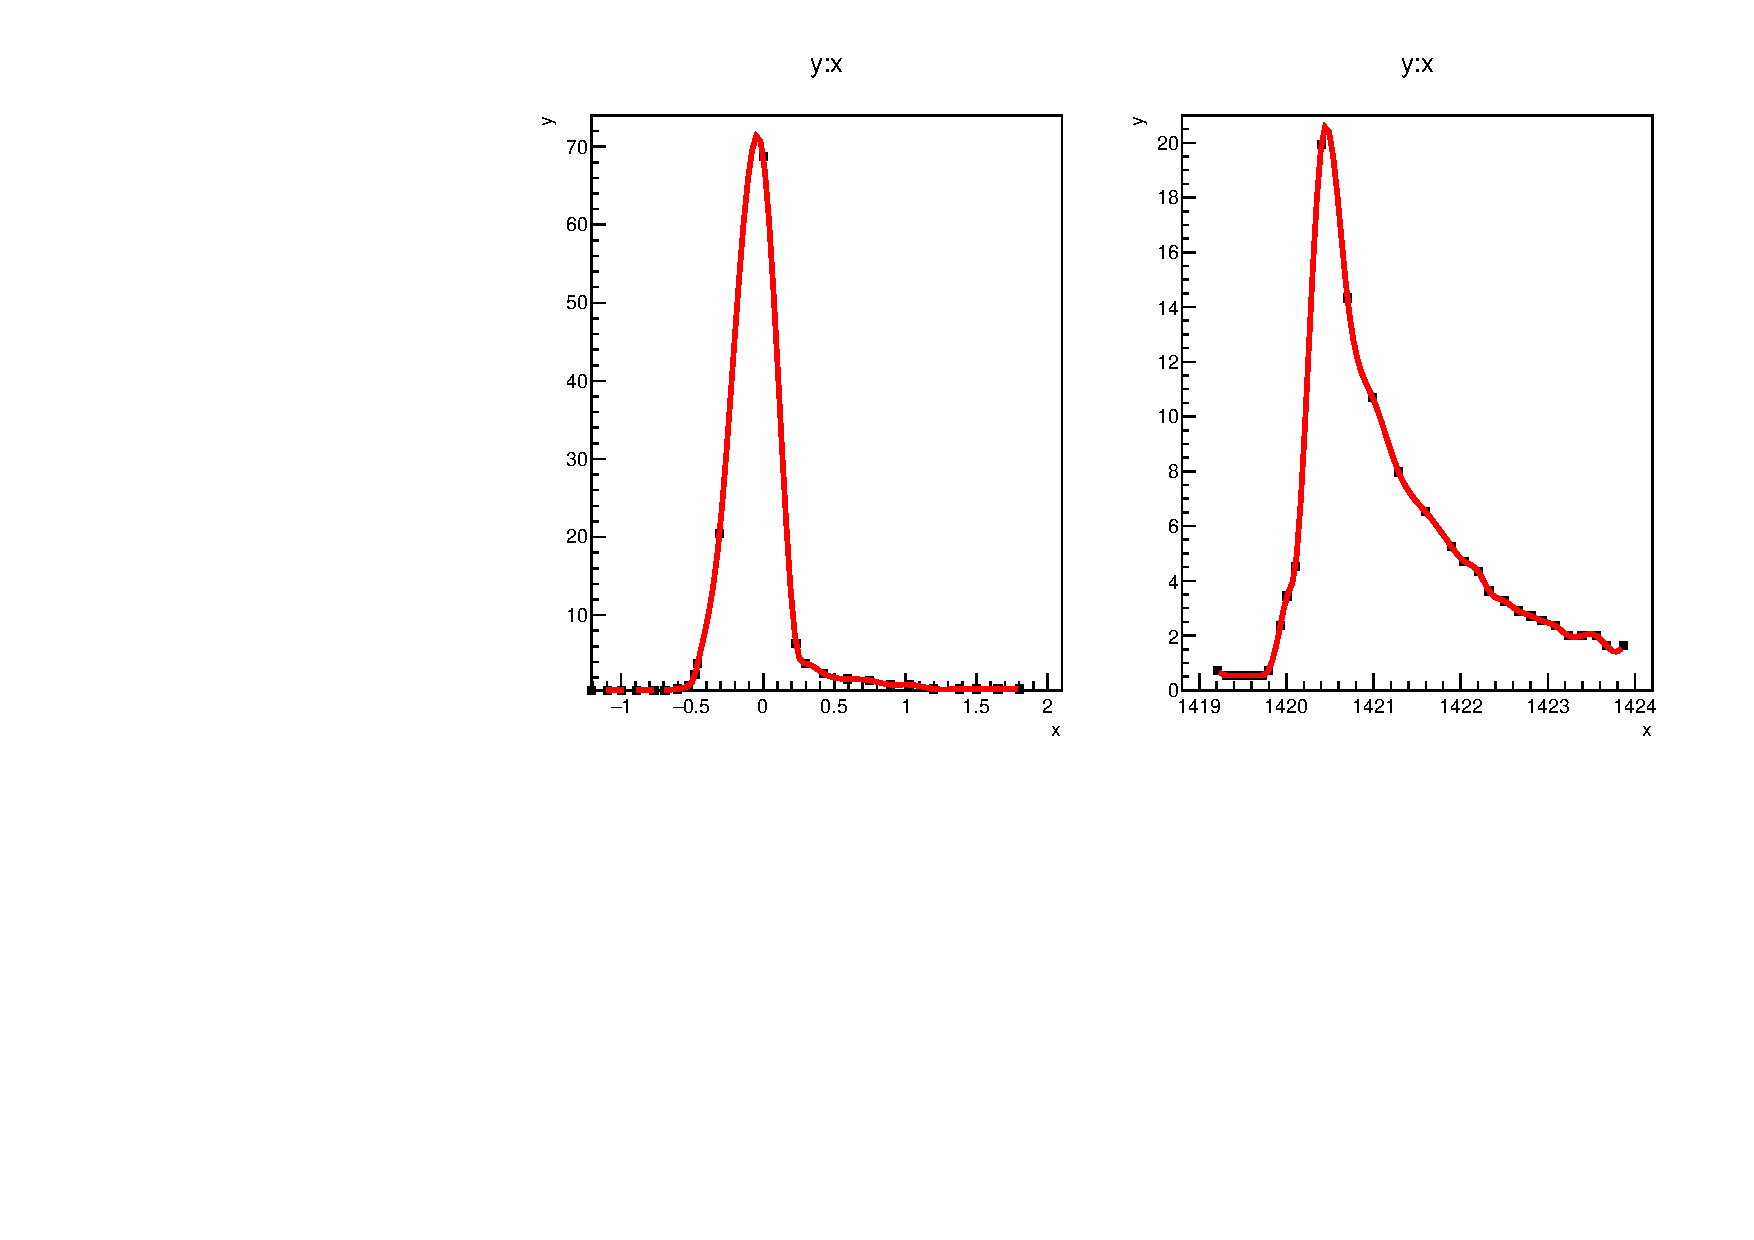
\includegraphics[width = \textwidth]{SplineInterpolation.pdf}
\caption{Data Obtained with PlotDigitizer}
\end{figure}
\end{frame}

\begin{frame}{ Probability $pMix = 50 \% $}
\begin{figure}[hbtp]
\centering
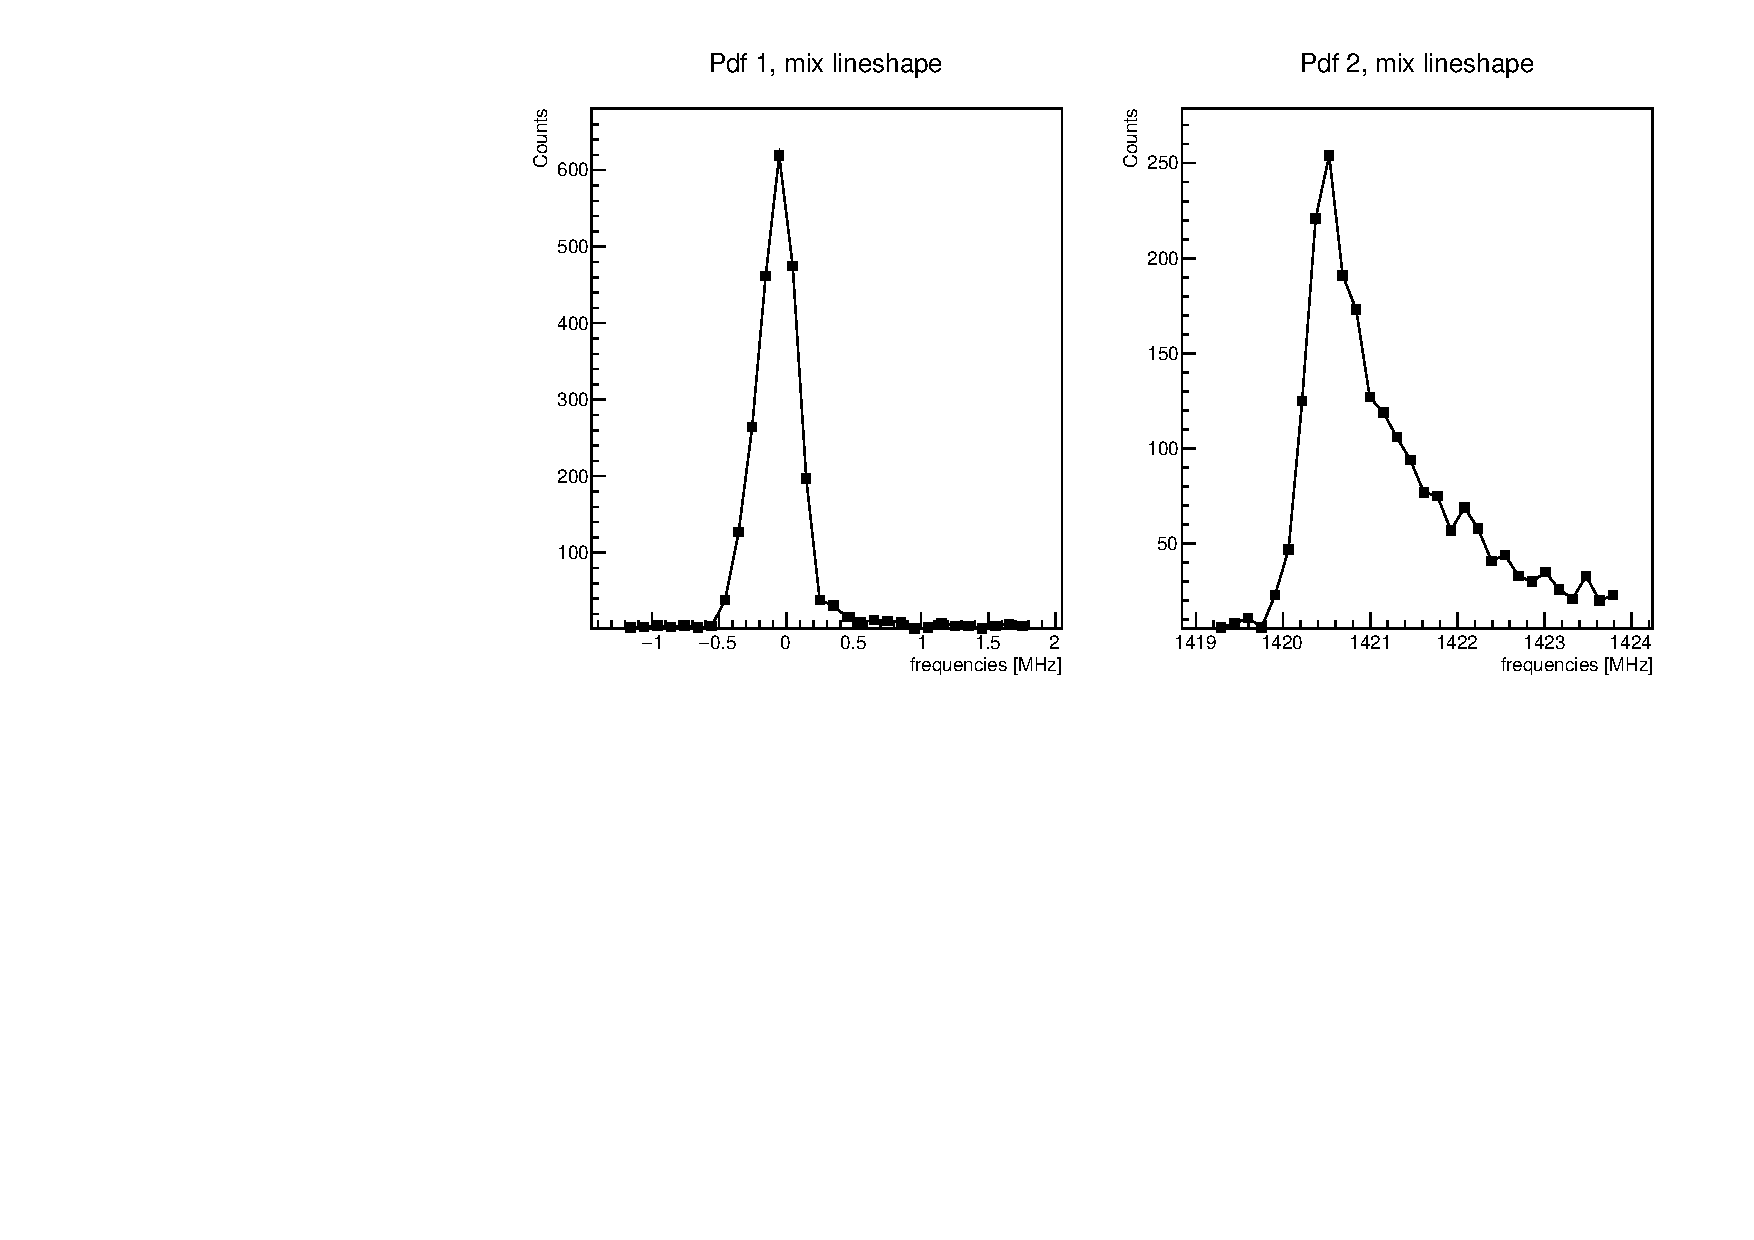
\includegraphics[width = \textwidth]{NmixOnly.pdf}
\caption{Events per frequence generated with the Pdf 1 (left) and Pdf 2 (right). \newline The Data include \textbf{only} the annihilation on the walls (mixing).}
\end{figure}
\end{frame}


\end{document}